\documentclass[conference]{IEEEtran}
\IEEEoverridecommandlockouts
% The preceding line is only needed to identify funding in the first footnote. If that is unneeded, please comment it out.
\usepackage{cite}
\usepackage{amsmath,amssymb,amsfonts}
\usepackage{algorithmic}
\usepackage{graphicx}
\usepackage{textcomp}
\usepackage{lipsum}
\usepackage{xcolor}
\usepackage{hyperref}
\def\BibTeX{{\rm B\kern-.05em{\sc i\kern-.025em b}\kern-.08em
    T\kern-.1667em\lower.7ex\hbox{E}\kern-.125emX}}
\begin{document}

\title{Synergy of Distributed Ledger Technologies and the Internet of Things*\\
% {\footnotesize \textsuperscript{*}Note: Sub-titles are not captured in Xplore and
% should not be used}
% \thanks{Identify applicable funding agency here. If none, delete this.}
}

\author{\IEEEauthorblockN{Sebastian Kanz}
\IEEEauthorblockA{\textit{Blockchain Engineer}\\
\textit{Distributed Ledger Technologies}\\
\textit{MaibornWolff GmbH}\\
Frankfurt am Main, Germany \\
sebastian.kanz@maibornwolff.de}
% \and
% \IEEEauthorblockN{2\textsuperscript{nd} Given Name Surname}
% \IEEEauthorblockA{\textit{dept. name of organization (of Aff.)} \\
% \textit{name of organization (of Aff.)}\\
% City, Country \\
% email address or ORCID}
% \and
% \IEEEauthorblockN{3\textsuperscript{rd} Given Name Surname}
% \IEEEauthorblockA{\textit{dept. name of organization (of Aff.)} \\
% \textit{name of organization (of Aff.)}\\
% City, Country \\
% email address or ORCID}
}

\maketitle

\begin{abstract}
  Manufacturers of household appliances have different opportunities to sell or rent their devices not exclusively to private consumers but also to companies and the gastronomic environment. Transforming those devices into IOT devices by making them ''smart'' with the concept of a ''digital twin'' enables manufacturers to utilize new technology and offer new payment models to their customers. This allows the development of an ecosystem in which new business processes can emerge and serveral stakeholders can participate: A platform that connects those smart devices and handles the communication, data persistency, security and the automated processing of the business logic. An evident approach for a suitable solution to create such a platfrom might be the application of blockchain technology - or in general the distributed ledger technology. Due to their characteristics like distribution, no-trust environment, integrity of data and the ability of automated code-processing it is worth investigating on that topic.\\ 
  In this paper the synergy between IOT and DLT is shown by the analyzation of a representative, practical IOT use case and the prototypical implementation based on the blockchain platform Ethereum.\\

  \cite{cisco2016}
  % The telecommunications company Cisco predicts that by 2030, more than 500 billion IOT devices connected to the Internet will have found their way into various areas of our daily lives \cite{cisco2016}. Networked objects of our everyday life such as refrigerators, coffee machines, the automated supply chain from the business environment or a smart city are only a few examples of this business field. Although the concept of IOT is still very theoretical, several use cases have already been developed. In order to fully exploit the great potential of IOT and to implement corresponding visions, a suitable IT solution must be provided for the corresponding use case. Many different manufacturers and service providers need a uniform platform on which they can network their IOT devices, services, business logic and customers with each other and integrate a secure payment system. The question arises whether and to what extent the two innovative technologies DLT and IOT can benefit from each other and whether DLT is suitable as a scaling, high-performance and secure technology for IOT use cases. To answer this question, this paper examines an exemplary IOT use case, creates a requirements analysis and determines a suitable DLT for validating the research question by means of a market analysis and a requirements assessment. Finally, the implementation of an exemplary prototype based on the selected DLT is used to validate the results of this thesis.
\end{abstract}

\begin{IEEEkeywords}
Blockchain, Distributed Ledger Technologies, Internet of Things, State Channel
\end{IEEEkeywords}


\section{Pay-As-You-Use renting of smart gastronomy devices}
The use case investigated in this paper is as follows:\\
Manufacturers offer their smart household appliances on a platform where customers can rent those devices and pay for the usage by a pay-as-you-use payment model. Therefore the devices have onboard sensors which are able to track and analyze the usage and the internal machine state. Furthermore other stakeholders like service-providers or suppliers take part on the platform and offer their services. The renting contracts as well as the service contracts - like the service provided by the service-provider or the supply contract for supplying customers with goods - is automatically processed by the platform. This includes the communication with the devices and their onboard sensors, the payment for consuming services and goods and the information providing to the involved stakeholders.\\
The present use case focuses on smart coffee machines rented to companies. Imagine the following setup: A company - here in the role of a customer - has an active renting contract with the manufacturer. The supplier is commissioned to deliver the machine as well as optinal goods to the customer. The payment and the delivery tracking are defined through the supply contract which is processed by the platform. As soon as the machine is plugged in at the customer's office and connected to the internet, the employees of the customer can order their coffee. They can authorize as company employees and pay the coffee with their company-wallet via a smartphone app - the communication between their smartphone and the coffee machine is done through near field communication (NFC). The coffee machine is able to check whether the company has enough credits for the coffee to be served. If the machine requires maintenance or if an error occures the service-provider is contacted. This process as well as the payment to the service-provider is fully automated through the platform. \\
The design of the present use case requires the platform to implement a set of features. To find a suitable platform solution the key requirements were elaborated and transferred into the DLT context:\\
\begin{itemize}
  \item Smart-contracts allow automated information processing on-chain.
  \item Oracle-services provide off-chain information to the DLT.
  \item Payment is needed for processing invoices of services and goods.
  \item Asynchronicity empowers IOT use cases.
  \item Performance is needed by every application and adjusted to the specific use case.
  \item Encryption needs to be ensured to protect customer data and privacy.
\end{itemize}

performance

For the evaluation the security and encryption mechanisms in DLTs reference is made to [XYZ]. Those topics are evaluated in detail in the given references and are not in the focus of this paper. The integration of payment can be done via a third-party or by built-in DLT functionality like cryptocurrency or tokens (see [XYZ]).\\
An important concept that needs to be mentioned is the smart-contract which enables this use case to be fully automated and process contracts and contract-logic onchain as well as providing oracle-services. Due to the fact that most modern DLTs offer smart-contract functionality this topic is not investigated on in detail. The key concept that empowers this use case is the need of asynchroneous communication and information processing. Most IOT use cases have too few ressources for providing user-friendly synchroneous communication. Due to connection-loss, power-outage or less computing ressources IOT devices can not guarantee a constant communication channel to other devices. Pushing the concept of asynchronicity a little further and increasing the out time between connections this is referred to as offline capability. To be able to offer the customers a satisfying user-experience the most critical point is the user interaction - in this usecase namely the serving of the coffee. If this process takes to long or aborts due to errors, the customers will decline the use case and the acceptance decreases as well as the economic efficiency.\\
Therefore technology of the underlying platform needs a mechanism for this offline functionality: The processing, the payment and the synchronization needs to take place in different time intervals. DLTs as a possible, modern solution offer so called state channels to tackle this issue. With offline communication, hashing and signing algorithms and the utilization of smart-contracts DLTs can ensure security, data integrity and payment processing in this scenario. The concept of state-channels is examined in detail in the following section.\\

\subsection{State channels for empowering and scaling IOT use cases}
Blockchains (4) are a compromise due to their nature. Due to the consensus protocol, independent of block size and network capacitya, a natural limit is given: For example, the Bitcoin network is limited on a block time of 10 minutes by the complex calculation of Proof-of-Work (PoW). If the block size is very small, blocks are propagated very quickly over the network, but only a few transactions can be transferred at once. If the block size is very large, it is very difficult for nodes to synchronize but more transactions can be transferred at once. This limitation of block size and block duration means that in the case of Bitcoin currently (as of 01/2020) on average about 7 transactions per second are possible (30).\\
Other implementations may use other consensus mechanisms and other parameters, but there are also natural barriers there. It becomes clear that with increasing demands mainly to transaction processing per time interval (mostly transactions per second (TPS)) improved performance and new solutions become necessary. (30)\\
As a possible answer to the scaling problem of blockchains so-called state channels were developed. The aim is to be able to transmit any kind of off-chain processing of status-changing operations, which are typically processed and stored on-chain. Thus the number of of transactions can be reduced and the interaction time between involved parties can be improved. In the context of payments, so-called micro-payments are made possible. State channels, which are limited to payment processing, are called payment channels. These can be faster and cheaper than normal transactions take place. The costs of such micro-payments can be kept very low, since not all transactions must be stored on-chain. (15)\\
Another big advantage of state channels is the empowerment of asynchroneous transactions. If participants are not in the blockchain network (e.g. due to connectivity problems), then no transactions are carried out. If real-world actions like the opening of a barrier or the processing of an action are dependant from an on-chain status update, then with loss of connectivity the real process will stand still until the connection is restored. State-channels could be used here in order to create an alternative processing that can also be used when the blockchain is not reachable. Some example implementations of state channels are Bitcoin's Lightning Network (34), Ethereum's Raiden Network or the implementation of Neo called Trinity (41).\\


\subsection{A practical realization of one-way payment-channels with IOT devices}
The payment-channels in this usecase are implemented as smart-contracts on the Ethereum blockchain. When a user submits to a rental offering and the renting contract is created, the corresponding smart-contract, that models a rental agreement, creates the data structure on-chain and initializes a payment agreement that is designed by a separate smart-contract. This creates the payment-channel between the involved parties and holds all relevant data.\\
Initially the payment-channel between the coffee machine and the customer is charged with a predefined amount of credits transferred on contract creation. The payment-channel is implemented as a one-way payment-channel, because the value is exchanged only to the wallet of the machine. Credits that remain in the channel after the machine closes the channel will be transferred back to the customer. Apart from the general concept of payment-channels, the present one implements a redeem function that pays out the transferred credits the receivers. Due to this functionality the payment-channels can be reused and recharged and do not need to be recreated; this is for performance and cost issues.\\
While the payment agreement data structure is an on-chain information container for the payment-channel, the communication between the participants happens off-chain. The data is only needed for data persistency purposes and for synchronization of the participants. To be able to transfer data from the coffee machines to the employees and back there must be a communication channel besides the blochchain. This is implemented by exchanging data via NFC: After pressing the coffee serving button, the coffee machine sends the payment data as a receipt via NFC to the employee's smartphone. The data is signed with the employee's private key and sent back from the smartphone to the coffee machine. The machine is able to verify the signature and persists the latest receipt locally. This process can be repeated as many times as there are enough credits in the payment-channel. Because there might occure a connection-loss the coffee machine might not be able to check the balance on-chain and has to rely on its local information. Because the payment-channels are one-way, there is no possibility for the customer to pay out his own credits and order a new coffee while the machine is offline. This must be ensured to avoid data inconsistency.\\
If the balance of the payment-channel reaches a critical threshold or a defined time interval is reached, the machine redeems the receipts and the money is transferred on-chain. The customer - in this use case the company or an authorized employee - can charge the payment-channel again to order more coffee in the future.\\
The described payment process with the utilization of the payment-channel as part of the renting agreement can be transferred to the other payment processes between more stakeholders like the service-provider mentioned above. The base concept and implementation remain the same.

\subsection{Architectural overview of involved components}
The present use case was evaluated by a prototypical implementation with the Ethereum blockchain. The focus of this was to show the general feasability and the synergy between DLT and IOT. The use case is not covered as a whole as this is not needed to approve the benefits of DLT for IOT use cases.\\

\begin{figure}[htbp]
 \centering
 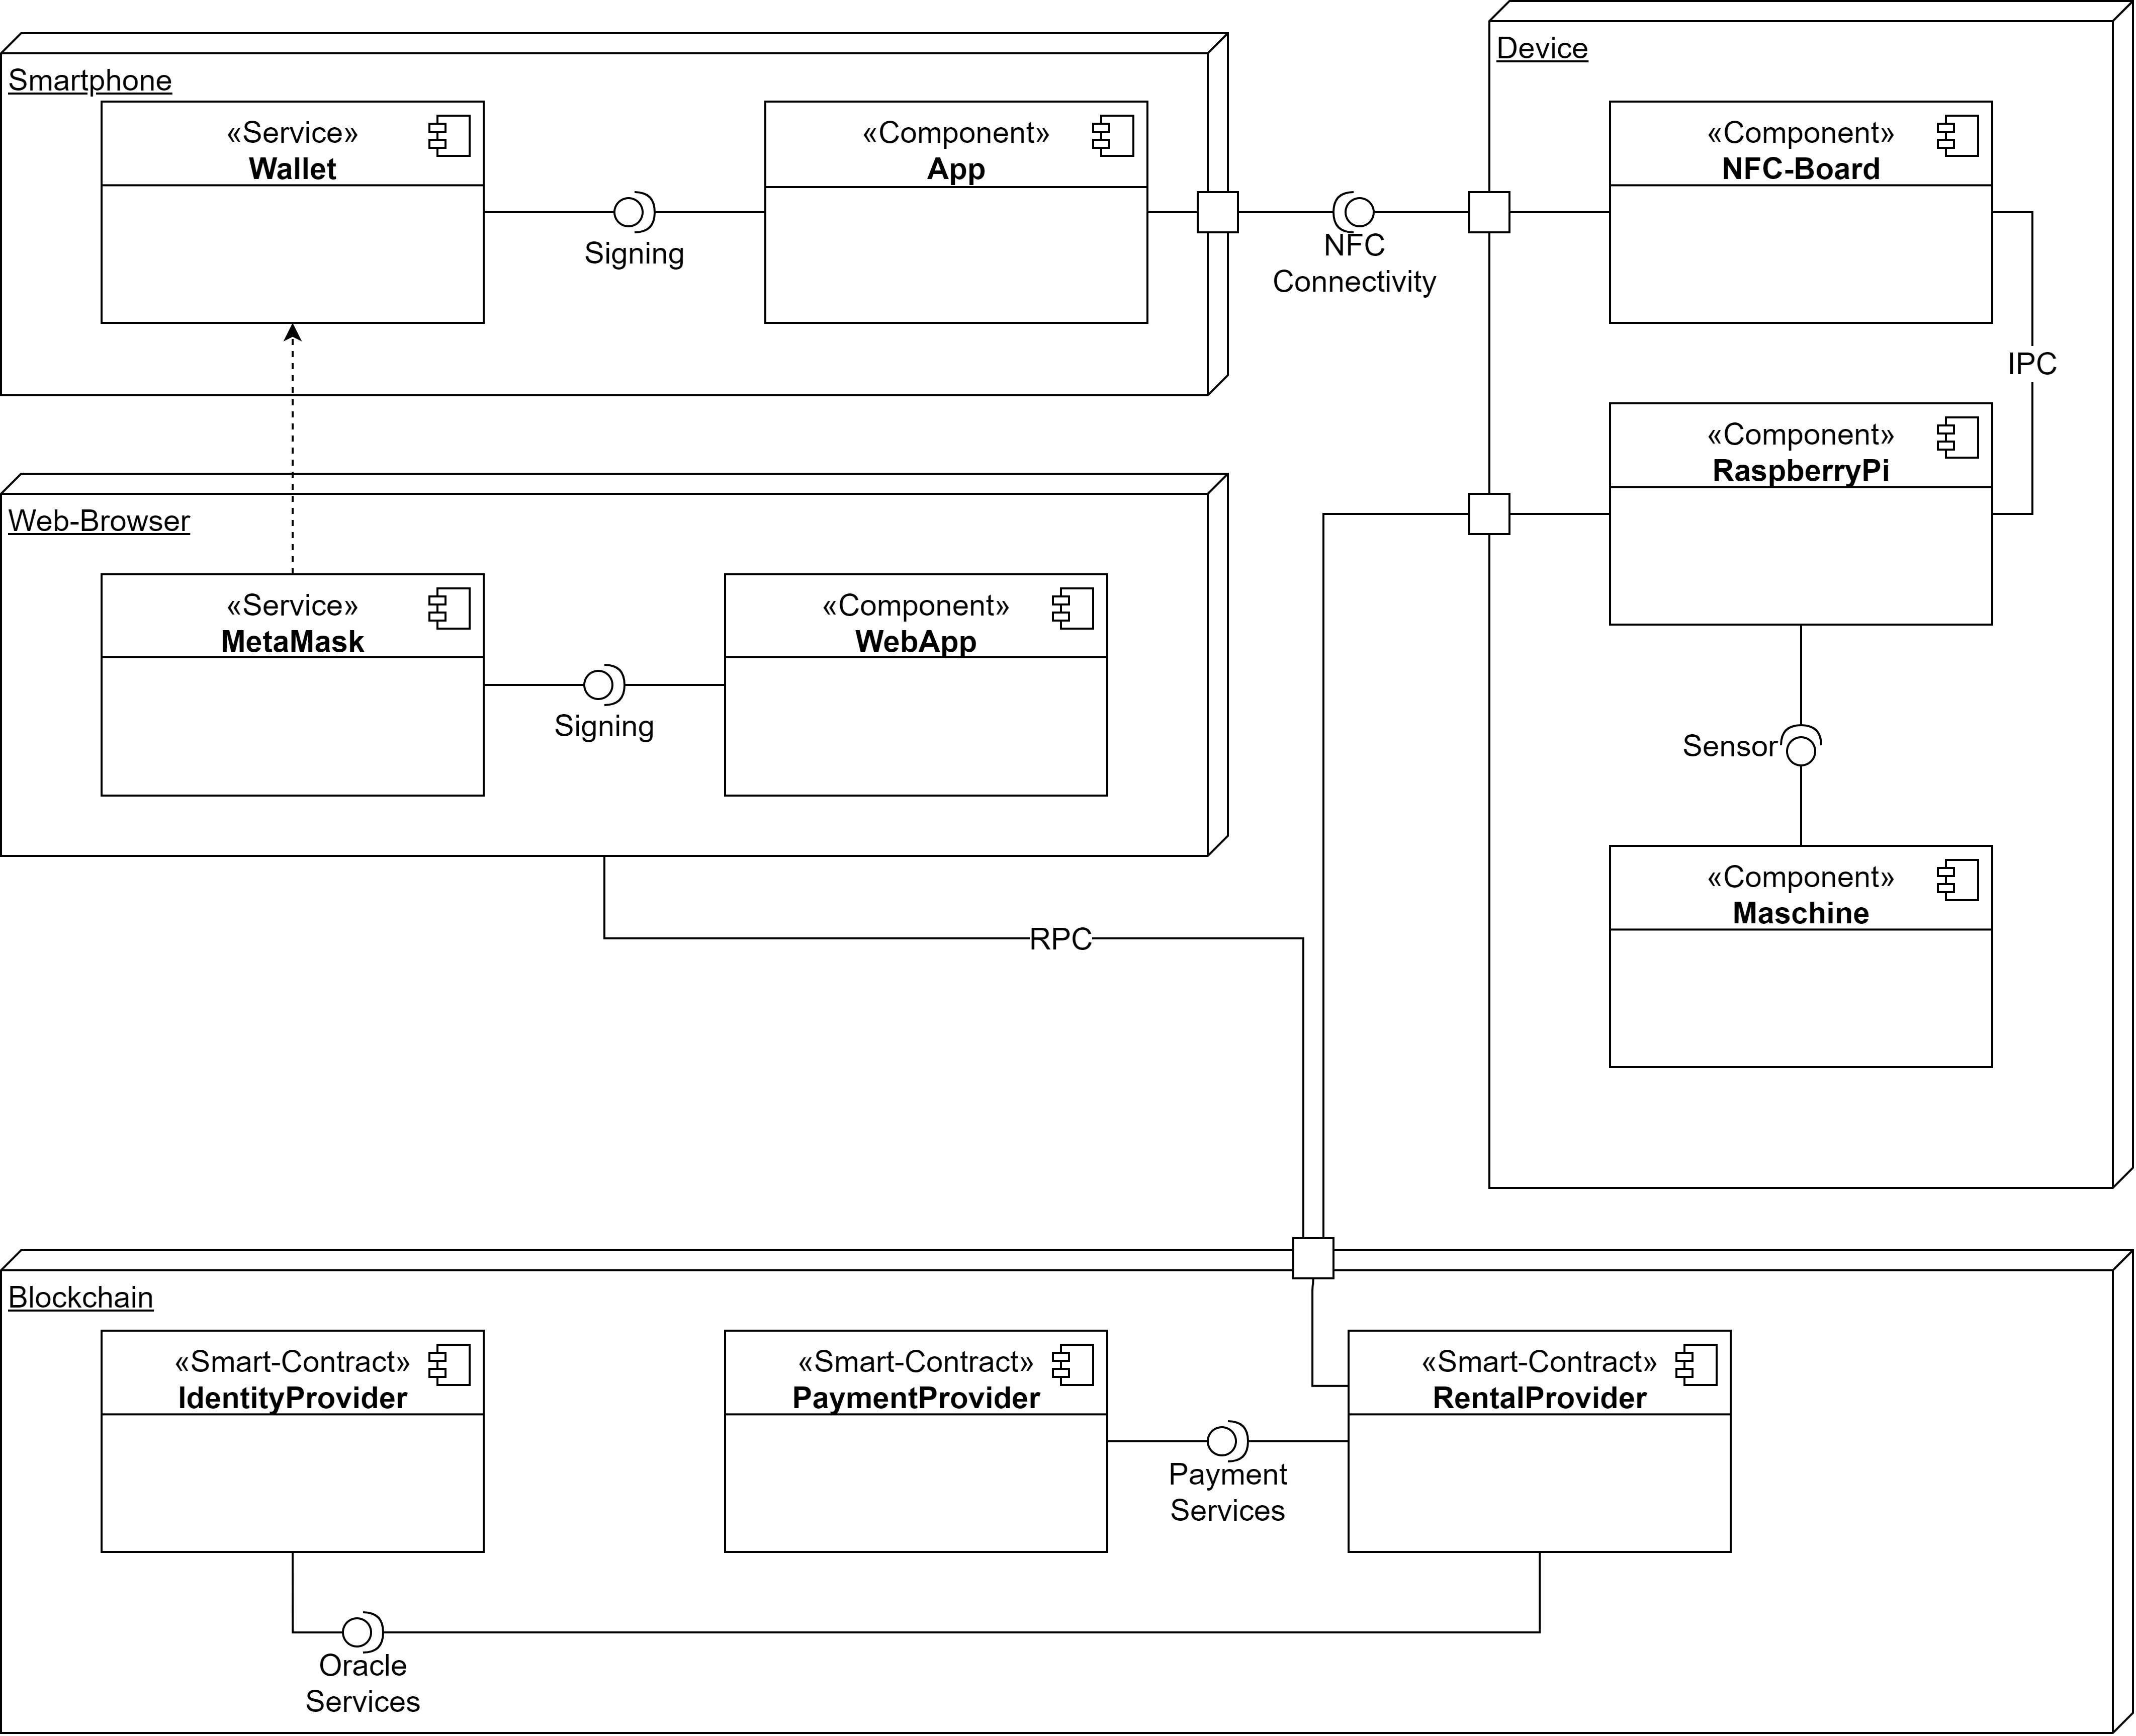
\includegraphics[width=0.4\textwidth]{media/Architecture.png}
 \caption{UML components diagramm; architectural overview}
 \label{fig:architecture}
\end{figure}

An overview of the application's architecture is shown in figure \ref{fig:architecture}. On-chain information is processed and stored via three smart-contracts: The IdentityProvider takes care of the contracting parties and manages access control. The PaymentProvider holds the payment-channels for the renting contracts and handles payment processing. The RenalProvider models the rental contracts on-chain and controls and calls the other smart-contracts.\\
Information on rentable devices, active contracts, contract handling and payment is accessable by all participants through a web app. The browser-integrated wallet MetaMask is used to sign and verify transactions to and from the blockchain.\\
To interact with the coffee machine the customer needs a smartphone with enabled NFC service. A mobile app enables the customer to authorize payments and sign incoming receipts from the coffee machine via NFC. The wallet used on the smartphone is the same as the one in the browser, so all information and contracting can be done across device boundaries.\\
To upgrade coffee machines and make them smart (as long as they do not support smart functionality out of the box) a RaspberryPi mini-computer is used in conjunction with a NFC breakout-board. This board is used for communication between the coffee machine and the smartphone. To measure the internal device state and gather usage data the device needs onboard sensors which must be available for the RaspberryPi to call (e.g. via REST or hardware-near protocols like I2C). The RaspberryPi itself can call the blockchain to redeem the receips or to report errors or request service inquiry.\\



\section{Results}
\textit{\lipsum[1-1]}
With the successful implementation of this usecase the general feasability is shown. IOT use cases can benefit from 

\subsection{Operating costs}
The use case is calculated as an industry-realistic quantity structure for the German market based on customer experience of MaibornWolff GmbH. The following numbers and data are based on the tests from the protoype or marked as assumptions.\\
A final configuration level of the present use case might include a total of 10.000 coffee machines on rent and 40 employees per office on average as well as a per capita consumption per year of coffee 164 litres.\\
At the time of calculating the Ethereum price was at 196,04 €/ETH; the GAS price is set to 5 GWEI. A more detailed overview of the assumptions made and the underlying data is shown in the appendix.\\


\subsection{Performance}

\subsection{Security}

\subsection{Privacy}



\section{Conclusion}
The implementation has been successful; a suitable implementation has been made, which prototypically evaluates the use case on the basis of Ethereum. A general statement for the entire IOT application area is thus not made and cannot be fully validated.  Use cases that show similar characteristics as the present implementation can profit with a high degree of certainty from a DLT implementation and the associated advantages. On the other hand, time-critical or performance-heavy IOT applications that cannot be implemented on the basis of a DLT because, for example, the required real-time communication is not available. In addition, applications that affect only a single stakeholder or are only executed at a single location are not designed for DLTs either, as they cannot benefit from the decentralized and no-trust environment.

\section{Future Work}
\textit{\lipsum[1-1]}

\section*{Acknowledgment}
\textit{\lipsum[1-1]}



\bibliographystyle{IEEEtran}
\bibliography{IEEEfull,references}

\end{document}
